\documentclass[11pt,]{article}
\usepackage{lmodern}
\usepackage{amssymb,amsmath}
\usepackage{ifxetex,ifluatex}
\usepackage{fixltx2e} % provides \textsubscript
\ifnum 0\ifxetex 1\fi\ifluatex 1\fi=0 % if pdftex
  \usepackage[T1]{fontenc}
  \usepackage[utf8]{inputenc}
\else % if luatex or xelatex
  \ifxetex
    \usepackage{mathspec}
  \else
    \usepackage{fontspec}
  \fi
  \defaultfontfeatures{Ligatures=TeX,Scale=MatchLowercase}
  \newcommand{\euro}{€}
    \setmainfont[]{IPAPMincho}
    \setsansfont[]{IPAPGothic}
\fi
% use upquote if available, for straight quotes in verbatim environments
\IfFileExists{upquote.sty}{\usepackage{upquote}}{}
% use microtype if available
\IfFileExists{microtype.sty}{%
\usepackage{microtype}
\UseMicrotypeSet[protrusion]{basicmath} % disable protrusion for tt fonts
}{}
\usepackage[margin=1in]{geometry}
\usepackage{hyperref}
\PassOptionsToPackage{usenames,dvipsnames}{color} % color is loaded by hyperref
\hypersetup{unicode=true,
            pdftitle={平成28年度社会医学実習--実施例},
            pdfauthor={王 超辰},
            colorlinks=true,
            linkcolor=blue,
            citecolor=Blue,
            urlcolor=Blue,
            breaklinks=true}
\urlstyle{same}  % don't use monospace font for urls
\usepackage{color}
\usepackage{fancyvrb}
\newcommand{\VerbBar}{|}
\newcommand{\VERB}{\Verb[commandchars=\\\{\}]}
\DefineVerbatimEnvironment{Highlighting}{Verbatim}{commandchars=\\\{\}}
% Add ',fontsize=\small' for more characters per line
\usepackage{framed}
\definecolor{shadecolor}{RGB}{248,248,248}
\newenvironment{Shaded}{\begin{snugshade}}{\end{snugshade}}
\newcommand{\KeywordTok}[1]{\textcolor[rgb]{0.13,0.29,0.53}{\textbf{{#1}}}}
\newcommand{\DataTypeTok}[1]{\textcolor[rgb]{0.13,0.29,0.53}{{#1}}}
\newcommand{\DecValTok}[1]{\textcolor[rgb]{0.00,0.00,0.81}{{#1}}}
\newcommand{\BaseNTok}[1]{\textcolor[rgb]{0.00,0.00,0.81}{{#1}}}
\newcommand{\FloatTok}[1]{\textcolor[rgb]{0.00,0.00,0.81}{{#1}}}
\newcommand{\ConstantTok}[1]{\textcolor[rgb]{0.00,0.00,0.00}{{#1}}}
\newcommand{\CharTok}[1]{\textcolor[rgb]{0.31,0.60,0.02}{{#1}}}
\newcommand{\SpecialCharTok}[1]{\textcolor[rgb]{0.00,0.00,0.00}{{#1}}}
\newcommand{\StringTok}[1]{\textcolor[rgb]{0.31,0.60,0.02}{{#1}}}
\newcommand{\VerbatimStringTok}[1]{\textcolor[rgb]{0.31,0.60,0.02}{{#1}}}
\newcommand{\SpecialStringTok}[1]{\textcolor[rgb]{0.31,0.60,0.02}{{#1}}}
\newcommand{\ImportTok}[1]{{#1}}
\newcommand{\CommentTok}[1]{\textcolor[rgb]{0.56,0.35,0.01}{\textit{{#1}}}}
\newcommand{\DocumentationTok}[1]{\textcolor[rgb]{0.56,0.35,0.01}{\textbf{\textit{{#1}}}}}
\newcommand{\AnnotationTok}[1]{\textcolor[rgb]{0.56,0.35,0.01}{\textbf{\textit{{#1}}}}}
\newcommand{\CommentVarTok}[1]{\textcolor[rgb]{0.56,0.35,0.01}{\textbf{\textit{{#1}}}}}
\newcommand{\OtherTok}[1]{\textcolor[rgb]{0.56,0.35,0.01}{{#1}}}
\newcommand{\FunctionTok}[1]{\textcolor[rgb]{0.00,0.00,0.00}{{#1}}}
\newcommand{\VariableTok}[1]{\textcolor[rgb]{0.00,0.00,0.00}{{#1}}}
\newcommand{\ControlFlowTok}[1]{\textcolor[rgb]{0.13,0.29,0.53}{\textbf{{#1}}}}
\newcommand{\OperatorTok}[1]{\textcolor[rgb]{0.81,0.36,0.00}{\textbf{{#1}}}}
\newcommand{\BuiltInTok}[1]{{#1}}
\newcommand{\ExtensionTok}[1]{{#1}}
\newcommand{\PreprocessorTok}[1]{\textcolor[rgb]{0.56,0.35,0.01}{\textit{{#1}}}}
\newcommand{\AttributeTok}[1]{\textcolor[rgb]{0.77,0.63,0.00}{{#1}}}
\newcommand{\RegionMarkerTok}[1]{{#1}}
\newcommand{\InformationTok}[1]{\textcolor[rgb]{0.56,0.35,0.01}{\textbf{\textit{{#1}}}}}
\newcommand{\WarningTok}[1]{\textcolor[rgb]{0.56,0.35,0.01}{\textbf{\textit{{#1}}}}}
\newcommand{\AlertTok}[1]{\textcolor[rgb]{0.94,0.16,0.16}{{#1}}}
\newcommand{\ErrorTok}[1]{\textcolor[rgb]{0.64,0.00,0.00}{\textbf{{#1}}}}
\newcommand{\NormalTok}[1]{{#1}}
\usepackage{graphicx,grffile}
\makeatletter
\def\maxwidth{\ifdim\Gin@nat@width>\linewidth\linewidth\else\Gin@nat@width\fi}
\def\maxheight{\ifdim\Gin@nat@height>\textheight\textheight\else\Gin@nat@height\fi}
\makeatother
% Scale images if necessary, so that they will not overflow the page
% margins by default, and it is still possible to overwrite the defaults
% using explicit options in \includegraphics[width, height, ...]{}
\setkeys{Gin}{width=\maxwidth,height=\maxheight,keepaspectratio}
\setlength{\parindent}{0pt}
\setlength{\parskip}{6pt plus 2pt minus 1pt}
\setlength{\emergencystretch}{3em}  % prevent overfull lines
\providecommand{\tightlist}{%
  \setlength{\itemsep}{0pt}\setlength{\parskip}{0pt}}
\setcounter{secnumdepth}{5}

%%% Use protect on footnotes to avoid problems with footnotes in titles
\let\rmarkdownfootnote\footnote%
\def\footnote{\protect\rmarkdownfootnote}

%%% Change title format to be more compact
\usepackage{titling}

% Create subtitle command for use in maketitle
\newcommand{\subtitle}[1]{
  \posttitle{
    \begin{center}\large#1\end{center}
    }
}

\setlength{\droptitle}{-2em}
  \title{平成28年度社会医学実習--実施例}
  \pretitle{\vspace{\droptitle}\centering\huge}
  \posttitle{\par}
  \author{王 超辰}
  \preauthor{\centering\large\emph}
  \postauthor{\par}
  \predate{\centering\large\emph}
  \postdate{\par}
  \date{2016年6月23日}


\usepackage{xltxtra}
\XeTeXlinebreaklocale ``ja''
\XeTeXlinebreakskip=0pt plus 1pt
\XeTeXlinebreakpenalty=0

% Redefines (sub)paragraphs to behave more like sections
\ifx\paragraph\undefined\else
\let\oldparagraph\paragraph
\renewcommand{\paragraph}[1]{\oldparagraph{#1}\mbox{}}
\fi
\ifx\subparagraph\undefined\else
\let\oldsubparagraph\subparagraph
\renewcommand{\subparagraph}[1]{\oldsubparagraph{#1}\mbox{}}
\fi

\begin{document}
\maketitle

\section{例:日本人肝がん罹患の年齢,出生コホート,時期効果分析}

\begin{Shaded}
\begin{Highlighting}[]
\NormalTok{## Load XLConnect}
\KeywordTok{library}\NormalTok{(XLConnect)}
\end{Highlighting}
\end{Shaded}

\begin{verbatim}
## Loading required package: XLConnectJars
\end{verbatim}

\begin{verbatim}
## XLConnect 0.2-11 by Mirai Solutions GmbH [aut],
##   Martin Studer [cre],
##   The Apache Software Foundation [ctb, cph] (Apache POI, Apache Commons
##     Codec),
##   Stephen Colebourne [ctb, cph] (Joda-Time Java library)
\end{verbatim}

\begin{verbatim}
## http://www.mirai-solutions.com ,
## http://miraisolutions.wordpress.com
\end{verbatim}

\begin{Shaded}
\begin{Highlighting}[]
\NormalTok{## From a newly created file with sheet 4 (rate data) only}
\NormalTok{rate.all <-}\StringTok{ }\KeywordTok{readWorksheetFromFile}\NormalTok{(}\StringTok{"cancer_incidence(1975-2011)rate.xls"}\NormalTok{,}
                                  \DataTypeTok{sheet =} \DecValTok{1}\NormalTok{)}
\NormalTok{## Change variable names}
\KeywordTok{names}\NormalTok{(rate.all) <-}\StringTok{ }\KeywordTok{gsub}\NormalTok{(}\StringTok{"X"}\NormalTok{, }\StringTok{"age"}\NormalTok{, }\KeywordTok{names}\NormalTok{(rate.all))}
\KeywordTok{names}\NormalTok{(rate.all) <-}\StringTok{ }\KeywordTok{gsub}\NormalTok{(}\StringTok{"歳"}\NormalTok{, }\StringTok{""}\NormalTok{, }\KeywordTok{names}\NormalTok{(rate.all))}
\KeywordTok{names}\NormalTok{(rate.all) <-}\StringTok{ }\KeywordTok{gsub}\NormalTok{(}\StringTok{"以上"}\NormalTok{, }\StringTok{"plus"}\NormalTok{, }\KeywordTok{names}\NormalTok{(rate.all))}
\KeywordTok{names}\NormalTok{(rate.all) <-}\StringTok{ }\KeywordTok{gsub}\NormalTok{(}\StringTok{"診断年"}\NormalTok{, }\StringTok{"Dia_yr"}\NormalTok{, }\KeywordTok{names}\NormalTok{(rate.all))}
\KeywordTok{names}\NormalTok{(rate.all) <-}\StringTok{ }\KeywordTok{gsub}\NormalTok{(}\StringTok{"}\CharTok{\textbackslash{}\textbackslash{}}\StringTok{."}\NormalTok{, }\StringTok{"_"}\NormalTok{, }\KeywordTok{names}\NormalTok{(rate.all))}
\NormalTok{## Show data}
\KeywordTok{head}\NormalTok{(rate.all)}
\end{Highlighting}
\end{Shaded}

\begin{verbatim}
##   コード   部位  ICD_10   性別 Dia_yr     粗率   age0_4   age5_9 age10_14
## 1      1 全部位 C00-C96 男女計   1975 184.6549 13.24920 8.021910 7.944879
## 2      1 全部位 C00-C96 男女計   1976 185.0981 13.14640 7.311146 7.597889
## 3      1 全部位 C00-C96 男女計   1977 189.4090 13.86778 7.400872 7.299964
## 4      1 全部位 C00-C96 男女計   1978 194.5231 13.11493 7.108764 6.130980
## 5      1 全部位 C00-C96 男女計   1979 206.5175 13.38973 6.660657 5.638117
## 6      1 全部位 C00-C96 男女計   1980 214.4543 14.02163 7.107233 6.551611
##    age15_19 age20_24 age25_29 age30_34 age35_39 age40_44 age45_49 age50_54
## 1  8.882128 13.18414 24.54009 41.92178 71.88043 128.1969 211.0058 300.2575
## 2  8.891426 11.32447 25.69828 38.42129 70.01396 125.0030 205.6629 296.9398
## 3 10.551438 10.42322 26.78686 38.13225 72.73761 125.9141 206.6744 297.4311
## 4 10.116003 10.40606 23.60261 38.56832 75.24708 126.1025 205.0247 308.5769
## 5  9.655429 11.11250 22.93809 41.57780 84.30307 127.7256 211.8893 326.0116
## 6  8.643361 12.09025 20.82652 43.88338 81.21430 127.6162 213.8217 327.8601
##   age55_59 age60_64 age65_69 age70_74 age75_79 age80_84 age85plus
## 1 430.9053 639.0219 884.1888 1173.113 1377.386 1360.574  1087.513
## 2 417.5249 618.8536 876.7602 1147.714 1389.089 1407.351  1121.981
## 3 405.1523 625.2349 895.6720 1114.264 1376.906 1431.072  1137.963
## 4 406.5789 621.4057 903.8451 1125.717 1400.840 1400.000  1208.894
## 5 438.9733 656.5278 910.9551 1170.201 1436.000 1442.207  1258.635
## 6 456.2925 656.3355 911.2209 1235.173 1448.579 1500.307  1314.581
\end{verbatim}

\subsection{Graphing hepatic cancer
data}\label{graphing-hepatic-cancer-data}

\begin{Shaded}
\begin{Highlighting}[]
\NormalTok{## Extract all-sex data hepatic cancer mortality data}
\NormalTok{rate.hepatic <-}\StringTok{ }\KeywordTok{subset}\NormalTok{(rate.all, 部位 ==}\StringTok{ "肝臓"} \NormalTok{&}\StringTok{ }\NormalTok{性別 ==}\StringTok{ "男女計"}\NormalTok{)}
\NormalTok{## Change to long format}
\KeywordTok{library}\NormalTok{(reshape2)}
\NormalTok{rate.hepatic.melt <-}\StringTok{ }\KeywordTok{melt}\NormalTok{(}\DataTypeTok{data          =} \NormalTok{rate.hepatic,}
                \NormalTok{##id.vars       = c(),}
                \DataTypeTok{measure.vars  =} \KeywordTok{names}\NormalTok{(rate.hepatic)[}\KeywordTok{grep}\NormalTok{(}\StringTok{"age"}\NormalTok{, }\KeywordTok{names}\NormalTok{(rate.hepatic))],}
                \DataTypeTok{variable.name =} \StringTok{"Age_Range"}\NormalTok{,}
                \DataTypeTok{value.name    =} \StringTok{"Incidence_Rate"}
                          \NormalTok{)}
\KeywordTok{names}\NormalTok{(rate.hepatic.melt$Age_Range) <-}\StringTok{ }\KeywordTok{gsub}\NormalTok{(}\StringTok{"_"}\NormalTok{, }\StringTok{"-"}\NormalTok{, }
                                           \KeywordTok{as.character}\NormalTok{(rate.hepatic.melt$Age_Range))}

\NormalTok{## Regroup calendar year of death by five year intervals}
\NormalTok{rate.hepatic.melt$Cal_yr5 <-}\StringTok{ }\KeywordTok{cut}\NormalTok{(rate.hepatic.melt$Dia_yr, }
                                 \DataTypeTok{breaks =} \KeywordTok{seq}\NormalTok{(}\DataTypeTok{from =} \DecValTok{1974}\NormalTok{, }\DataTypeTok{to =} \DecValTok{2015}\NormalTok{, }\DataTypeTok{by =} \DecValTok{5}\NormalTok{))}

\NormalTok{## Create a variable representing the lowest age in the interval}
\NormalTok{rate.hepatic.melt$age <-}\StringTok{ }\KeywordTok{seq}\NormalTok{(}\DataTypeTok{from =} \DecValTok{0}\NormalTok{, }\DataTypeTok{to =} \DecValTok{85}\NormalTok{, }
                             \DataTypeTok{by =} \DecValTok{5}\NormalTok{)[rate.hepatic.melt$Age_Range]}

\NormalTok{## Calculate the year of birth}
\NormalTok{rate.hepatic.melt$Birth_yr <-}\StringTok{ }\KeywordTok{with}\NormalTok{(rate.hepatic.melt, }
                                   \NormalTok{Dia_yr -}\StringTok{ }\NormalTok{age)}

\NormalTok{## Create the year of birth categories}
\NormalTok{rate.hepatic.melt$Birth_yr5 <-}\StringTok{ }\KeywordTok{cut}\NormalTok{(rate.hepatic.melt$Birth_yr,}
                                   \DataTypeTok{breaks =} \KeywordTok{seq}\NormalTok{(}\DataTypeTok{from =} \DecValTok{1889}\NormalTok{, }\DataTypeTok{to =} \DecValTok{2015}\NormalTok{, }\DataTypeTok{by =} \DecValTok{5}\NormalTok{))}
\NormalTok{rate.hepatic.melt$Birth_yr30 <-}\StringTok{ }\KeywordTok{cut}\NormalTok{(rate.hepatic.melt$Birth_yr,}
                                    \DataTypeTok{breaks =} \KeywordTok{seq}\NormalTok{(}\DataTypeTok{from =} \DecValTok{1870}\NormalTok{, }\DataTypeTok{to =} \DecValTok{2030}\NormalTok{, }\DataTypeTok{by =} \DecValTok{30}\NormalTok{))}

\NormalTok{## Check first 20 rows}
\KeywordTok{head}\NormalTok{(rate.hepatic.melt, }\DecValTok{20}\NormalTok{)}
\end{Highlighting}
\end{Shaded}

\begin{verbatim}
##    コード 部位 ICD_10   性別 Dia_yr      粗率 Age_Range Incidence_Rate
## 1       8 肝臓    C22 男女計   1975  9.679323    age0_4      0.6699593
## 2       8 肝臓    C22 男女計   1976 10.232036    age0_4      0.7111653
## 3       8 肝臓    C22 男女計   1977 10.302749    age0_4      0.6767309
## 4       8 肝臓    C22 男女計   1978 11.002483    age0_4      0.5081630
## 5       8 肝臓    C22 男女計   1979 11.981952    age0_4      0.3948111
## 6       8 肝臓    C22 男女計   1980 12.930932    age0_4      0.2818418
## 7       8 肝臓    C22 男女計   1981 14.055343    age0_4      0.2070898
## 8       8 肝臓    C22 男女計   1982 15.245212    age0_4      0.2383940
## 9       8 肝臓    C22 男女計   1983 16.551309    age0_4      0.1801106
## 10      8 肝臓    C22 男女計   1984 18.210172    age0_4      0.1572533
## 11      8 肝臓    C22 男女計   1985 19.452466    age0_4      0.2010923
## 12      8 肝臓    C22 男女計   1986 20.603754    age0_4      0.3281378
## 13      8 肝臓    C22 男女計   1987 22.210135    age0_4      0.3770423
## 14      8 肝臓    C22 男女計   1988 22.936400    age0_4      0.3876525
## 15      8 肝臓    C22 男女計   1989 23.603099    age0_4      0.2227171
## 16      8 肝臓    C22 男女計   1990 26.152168    age0_4      0.3234304
## 17      8 肝臓    C22 男女計   1991 27.076901    age0_4      0.4731861
## 18      8 肝臓    C22 男女計   1992 28.361939    age0_4      0.4672144
## 19      8 肝臓    C22 男女計   1993 28.694175    age0_4      0.6729033
## 20      8 肝臓    C22 男女計   1994 28.142745    age0_4      0.6448413
##        Cal_yr5 age Birth_yr   Birth_yr5          Birth_yr30
## 1  (1974,1979]   0     1975 (1974,1979] (1.96e+03,1.99e+03]
## 2  (1974,1979]   0     1976 (1974,1979] (1.96e+03,1.99e+03]
## 3  (1974,1979]   0     1977 (1974,1979] (1.96e+03,1.99e+03]
## 4  (1974,1979]   0     1978 (1974,1979] (1.96e+03,1.99e+03]
## 5  (1974,1979]   0     1979 (1974,1979] (1.96e+03,1.99e+03]
## 6  (1979,1984]   0     1980 (1979,1984] (1.96e+03,1.99e+03]
## 7  (1979,1984]   0     1981 (1979,1984] (1.96e+03,1.99e+03]
## 8  (1979,1984]   0     1982 (1979,1984] (1.96e+03,1.99e+03]
## 9  (1979,1984]   0     1983 (1979,1984] (1.96e+03,1.99e+03]
## 10 (1979,1984]   0     1984 (1979,1984] (1.96e+03,1.99e+03]
## 11 (1984,1989]   0     1985 (1984,1989] (1.96e+03,1.99e+03]
## 12 (1984,1989]   0     1986 (1984,1989] (1.96e+03,1.99e+03]
## 13 (1984,1989]   0     1987 (1984,1989] (1.96e+03,1.99e+03]
## 14 (1984,1989]   0     1988 (1984,1989] (1.96e+03,1.99e+03]
## 15 (1984,1989]   0     1989 (1984,1989] (1.96e+03,1.99e+03]
## 16 (1989,1994]   0     1990 (1989,1994] (1.96e+03,1.99e+03]
## 17 (1989,1994]   0     1991 (1989,1994] (1.99e+03,2.02e+03]
## 18 (1989,1994]   0     1992 (1989,1994] (1.99e+03,2.02e+03]
## 19 (1989,1994]   0     1993 (1989,1994] (1.99e+03,2.02e+03]
## 20 (1989,1994]   0     1994 (1989,1994] (1.99e+03,2.02e+03]
\end{verbatim}

\begin{Shaded}
\begin{Highlighting}[]
\NormalTok{## Load ggplot2}
\KeywordTok{library}\NormalTok{(ggplot2)}

\NormalTok{## Plot by calendar year, grouped by age of diagnosis}
\KeywordTok{ggplot}\NormalTok{(}\DataTypeTok{data =} \NormalTok{rate.hepatic.melt,}
       \DataTypeTok{mapping =} \KeywordTok{aes}\NormalTok{(}\DataTypeTok{x =} \NormalTok{Birth_yr, }\DataTypeTok{y =} \NormalTok{Incidence_Rate,}
                     \DataTypeTok{color =} \NormalTok{Age_Range)) +}\StringTok{ }
\StringTok{  }\KeywordTok{geom_line}\NormalTok{() +}
\StringTok{  }\KeywordTok{geom_point}\NormalTok{() +}
\StringTok{    }\KeywordTok{labs}\NormalTok{(}\DataTypeTok{title =} 
           \StringTok{"Hepatic Cancer Incidence in Japan}\CharTok{\textbackslash{}n}\StringTok{ (Grouped by age at diagnosis)"}\NormalTok{) +}\StringTok{ }
\StringTok{    }\KeywordTok{theme_bw}\NormalTok{() +}
\StringTok{    }\KeywordTok{theme}\NormalTok{(}\DataTypeTok{legend.key =} \KeywordTok{element_blank}\NormalTok{(),}
          \DataTypeTok{axis.text.x =} \KeywordTok{element_text}\NormalTok{(}\DataTypeTok{angle=}\DecValTok{90}\NormalTok{, }\DataTypeTok{vjust=}\DecValTok{1}\NormalTok{))}
\end{Highlighting}
\end{Shaded}

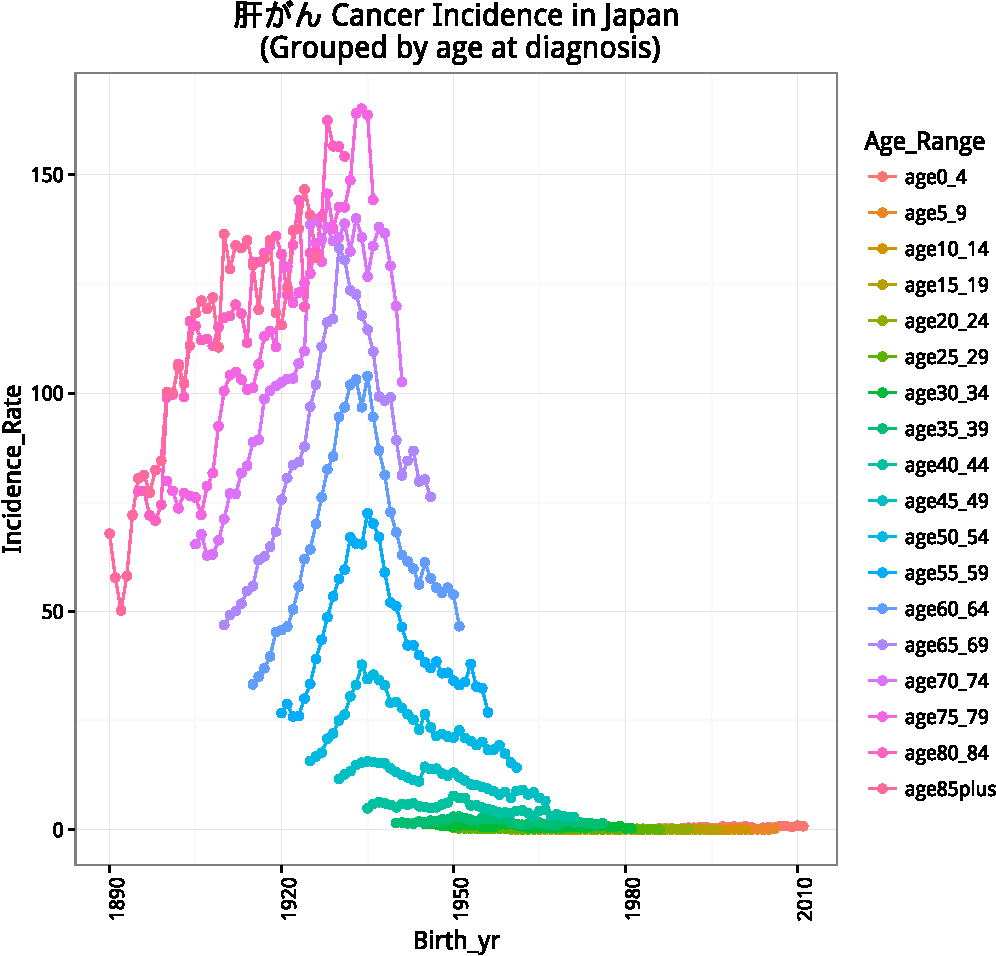
\includegraphics{example_files/figure-latex/unnamed-chunk-2-1.pdf}

\hypertarget{refs}{}

\end{document}
